\section{Instruction Memory}

The instruction Memory module stores the read-only instructions to be executed on the processor. The following subsections describe this module's design, implementation, and testing.

\subsection{Instruction Memory design}
\begin{figure}[H]
    \centering
    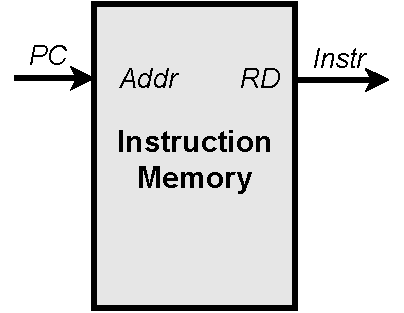
\includegraphics[width=.35\columnwidth]{pics/diagrams/riscv/modules/instruction_memory}
    \caption{Instruction Memory design}
    \label{fig:instruction_memory_module}
\end{figure}

\begin{itemize}
    \setlength\itemsep{3pt}
    \item \codeword{Addr} -- the address of the instruction to be read;
    \item \codeword{Instruction} -- the instruction read from the memory at the specified address.
\end{itemize}

\subsection{Instruction Memory implementation}

Since this memory is read-only, we hard-coded its contents in the module definition.

Data addressing is done byte-wise. Thus, given that instructions are 2 bytes long, we omit the first bit of the address when selecting the output (and so outputting the same instruction for both even and odd addresses).

We implemented such a behavior using the \codeword{case} statement:
\begin{code}[8]{Hard-coded Instruction example}
always @(Address) begin
case (Address[lv:1]) // Here we omit the first bit
    // This is the contents of the instruction memory
    00: Instruction = { 3'b011, 3'b000, 10'sd2 };
    ...
\end{code}

If the address goes out of the bounds of the memory, we return the default command, which does the multiplication of the $R_0$ by 1:
\begin{code}[17]{Default Instruction}
    ...
    default: Instruction = { 3'b001, 3'b000, 3'b000, 7'sd1 };
endcase
...
\end{code}

